%!TEX root = ../main.tex

% TODO: Writes something here!

\section{Validation}
% TODO: Write something here

\subsection{Seven Segments Display Example}
The seven segments example have been presented in different parts throughout this thesis. An illustration of the translated unclocked seven segments network can be seen in Figure \ref{fig:cspm-network}.\\

The unclocked \cspm{} network consists of 12 different processes, all created so that not only the network is simulated correctly, but also so the assertions we wish to make, are in place. The input is represented by a triangle, since it transpiles from an SME process to a \cspm{} channel. Each of the dotted squares represents the network of synchronizations for each \texttt{time} processes, which in itself is a process in \cspm{}. For each network, we have the \texttt{time} processes and two monitor processes, for example, $H$, $M_{H_1}$ and $M_{H_2}$.
\\

% Errornous example
\begin{listing}
\begin{minted}[escapeinside=||, mathescape=true]{cspm_lexer.py:CSPmLexer -x}
channel clock_out_val : {0..131071}

channel hours_out_first_digit : {0..3}
channel hours_out_second_digit : {0..15}
    |$\vdots$|

Hours(hours_in) =
let
    hours = hours_in / 3600
    |$\vdots$|

Hours_out_first_digit_monitor(c) =
    c ? x -> if 0 <= x and x <= 2 then SKIP else STOP
Hours_out_second_digit_monitor(c) =
    c ? x -> if 0 <= x and x <= 9 then SKIP else STOP

\end{minted}
\caption{Example of an erroneous version of the \texttt{Hours} process from the \cspm{} seven segment display example seen in Listing~\ref{lst:smeil} and in Listing~\ref{lst:cspm} in the appendix.}
\label{lst:cspm_error}
\end{listing}

In order to show that the verification is accurate, the example in Listing~\ref{lst:cspm_error} contains an error that results in FDR4 failing the verification. In Listing~\ref{lst:cspm_error} the example is only able to handle an input that is below 24 hours. This is because the calculation in the \texttt{Hours} process does not handle the wrap around at the 24\textsuperscript{th} hour. This means that if the input represents more than 24 hours, the assertions will fail in FDR4 because one seven segment display suddenly has to display two digits instead of one. An example of such could be the input \texttt{131071}, which represents 36 hours, 24 minutes and 31 seconds, or 1 day, 12 hours, 24 minutes and 31 seconds. When trying to assert the code from Listing~\ref{lst:cspm_error} in FDR4, the assertion fails. The counterexample shows that the number 3 is communicated on \texttt{hours\_out\_first\_digit}, which is not allowed according to the monitor process on lines 12 and 13 in Listing~\ref{lst:cspm_error}.\\

This example of failure shows how verifying the solution with a tool like FDR4 actually catches errors that the programmer might have overseen. In this case, the error is simply corrected by adding \texttt{\% 24} on the end of line 9 in Listing~\ref{lst:cspm_error} and can be seen corrected in Listing~\ref{lst:cspm} in the appendix at line 15. Now when we try to assert the example in FDR4, it passes. By using modulo on the result, we ensure that we still get the accurate time of day, no matter how many full days the input represents.
The full SMEIL and \cspm{} code for the unclocked seven segment display example can be seen in Listing~\ref{lst:smeil} and in Listing~\ref{lst:cspm} in the appendix.

\begin{figure}[!ht]
  \centering
  \begin{tikzpicture}
    \node [mytriangle] (I) at (0, 0) {$I$};

    %%%%

    \node [mycircle, above right=25ex and 25ex of I] (H) {$H$};

    \node [mysquare, above right=1.5ex and 25ex of H] (H_d1) {$D_{H_1}$};
    \node [mysquare, below right=1.5ex and 25ex of H] (H_d2) {$D_{H_2}$};
    \node [mycircle, above right=3ex and 7.5ex of H] (H_m1) {$M_{H_1}$};
    \node [mycircle, below right=3ex and 7.5ex of H] (H_m2) {$M_{H_2}$};
    \node [draw, red, thick, dotted, fit=(H)(H_m1)(H_m2), inner sep=0.5cm] {};
    \node [right=15ex of H, red] {$N_{hours}$};

    \draw [myarrow, smooth] (I) to[out=0, in=180] (H);

    \draw [myarrow, smooth] (H) to[out=0, in=180] coordinate[midway, black!50, draw, shape=circle, inner sep=0pt, minimum size=5pt](H_mp1) (H_d1);
    \draw (H_m1) -- (H_mp1)  [black!50];
    \draw [myarrow, smooth] (H) to[out=0, in=180] coordinate[midway, black!50, draw, shape=circle, inner sep=0pt, minimum size=5pt](H_mp2) (H_d2);
    \draw (H_m2) -- (H_mp2)  [black!50];

    %%%%

    \node [mycircle, right=23.2ex of I] (M) {$M$};

    \node [mysquare, above right=1.5ex and 25ex of M] (M_d1) {$D_{M_1}$};
    \node [mysquare, below right=1.5ex and 25ex of M] (M_d2) {$D_{M_2}$};
    \node [mycircle, above right=3ex and 7.5ex of M] (M_m1) {$M_{M_1}$};
    \node [mycircle, below right=3ex and 7.5ex of M] (M_m2) {$M_{M_2}$};
    \node [draw, red, thick, dotted, fit=(M)(M_m1)(M_m2), inner sep=0.5cm] {};
    \node [right=15ex of M, red] {$N_{minutes}$};

    \draw [myarrow, smooth] (I) to[out=0, in=180] (M);

    \draw [myarrow, smooth] (M) to[out=0, in=180] coordinate[midway, black!50, draw, shape=circle, inner sep=0pt, minimum size=5pt](M_mp1) (M_d1);
    \draw (M_m1) -- (M_mp1)  [black!50];
    \draw [myarrow, smooth] (M) to[out=0, in=180] coordinate[midway, black!50, draw, shape=circle, inner sep=0pt, minimum size=5pt](M_mp2) (M_d2);
    \draw (M_m2) -- (M_mp2)  [black!50];

    %%%%

    \node [mycircle, below right=24.5ex and 24.5ex of I] (S) {$S$};

    \node [mysquare, above right=1.5ex and 25ex of S] (S_d1) {$D_{S_1}$};
    \node [mysquare, below right=1.5ex and 25ex of S] (S_d2) {$D_{S_2}$};
    \node [mycircle, above right=3ex and 7.5ex of S] (S_m1) {$M_{S_1}$};
    \node [mycircle, below right=3ex and 7.5ex of S] (S_m2) {$M_{S_2}$};
    \node [draw, red, thick, dotted, fit=(S)(S_m1)(S_m2), inner sep=0.50cm, inner ysep=0.5cm] {};
    \node [right=15ex of S, red] {$N_{seconds}$};

    \draw [myarrow, smooth] (I) to[out=0, in=180] (S);

    \draw [myarrow, smooth] (S) to[out=0, in=180] coordinate[midway, black!50, draw, shape=circle, inner sep=0pt, minimum size=5pt](S_mp1) (S_d1);
    \draw (S_m1) -- (S_mp1)  [black!50];
    \draw [myarrow, smooth] (S) to[out=0, in=180] coordinate[midway, black!50, draw, shape=circle, inner sep=0pt, minimum size=5pt](S_mp2) (S_d2);
    \draw (S_m2) -- (S_mp2)  [black!50];
  \end{tikzpicture}
  \caption{A seven segment display clock network in \cspm{}. $I$ represents the input channel. $N_{hours}$, $N_{minutes}$ and $N_{seconds}$ represent the network processes with $H$, $M$ and $S$ as the \texttt{time} processes. The results from the \texttt{time} processes are communicated to the displays. The displays are represented by a square since they are not actual \cspm{} processes. Each display communication also has a monitor process which assert the legal communication values.}
  \label{fig:cspm-network}
\end{figure}


\subsection{Addone Example}
The \texttt{addone} example have been introduced in Chapter \ref{chap:clock} and as explained, it does not translate well in the initial version of TAPS. Illustrations of the clocked network with its monitor processes can be seen in Figure \ref{fig:addone_clocked_monitor} in Chapter \ref{chap:clock}.
The difference between a clocked an unclocked network is that FDR is able to verify different internal states in the clocked version which suits this cyclic network perfectly. Just as the seven segment example, there can be restrictions as to how much data the bus can represent but the values communicated on the \texttt{addone} network will increasse indefinitely unless restricted. The simulation ...

...it is not possible to represent indefinite numbers on is important to be able to verify...
The simulation of the original SMEIL network will of course only simulate a specific number of clock cycles and since the observed values are used for the verification, it is necessary to ensure the simulation represents the v
The monitor processes in the \texttt{addone} network verifies the communicated values the same way as the seven segments example

\section{Problem Size Experiments}
The examples presented in this thesis are not very complex, but they provide a suitable introduction to the translation and the verification in FDR4. More complex examples would have required a substantial introduction and it would not be as straightforward to understand the translations. The challenge with verification as the refinement check provided by FDR4 is to keep the verification time to a minimum. FDR4 performs different kinds of internal optimizations on the networks and it also provides several compression algorithms to provide feasible verification time to larger problems. \\

I have performed some experiments on the seven segments example to examine the verification time in FDR.
% TODO: Rewrite if I cannot use the unclocked version!
Both experiments have been run on a (info to come) machine with no other programs running. The experiments consists of meassuring three different properties of the FDR4 verification. The first property is \texttt{verification time} which is meassured by the \texttt{time} command. Even though all experiments have been performed on the same machine, to avoid potential confusion, the GNU \texttt{time} command was used istead of the build-in \texttt{time} command shells like bash and zsh provide. This property can provide an insight into the amount of time it takes for FDR4 to verify \cspm{} networks with different sizes of input.\\

The second property is \texttt{number of visited states} which is a piece of information FDR4 provides.
As explained in Chapter \ref{chap:background} FDR4 performs compression to minimise the state space. It is interesting to see if the verification time follows the number of visited states for the examples. This will give an insight into the inner workings of FDR4 and how the state space compression behaves.
Because the seven segments example is divided into three different assertions, one for each \texttt{time} process, FDR4 provides a seperate \texttt{number of visited states} for each verified \texttt{time} process. \\

The last property is \texttt{resident set size} which is also provided by the GNU \texttt{time} command. The resident set size defines how much memory the process currently has in main memory and it will provide an insight into how much memory FDR requires to verify the network. If FDR4 requires too much memory, it is not feasible to verify larger problems unless compression algorithms can reduce the state space. \\

The experiment have been designed to keep the internal system fixed and only increase the size of the input range for the system. This means that FDR4 will verify increasingly more values, but the network in itself stays the same.
The lower bound of the input range will be fixed at 0 and the upper bound will be increased with 500 for each verification until 15000. All three property values are gathered after FDR4 finish the verification.
This experiment will hopefully provide a simple understanding of how the state space evolves with the input range.
\subsection{Unclocked Experiment}
The full code for the unclocked seven segments display example can be seen in Listing \ref{lst:cspm} in Appendix %TODO: Figure out how this should be presented. One appendix or several?
The unclocked seven segments display example consists of three \texttt{time} processes with associated monitor processes. The number of states are in this example equal for each \texttt{time} process for each verified input and therefore this property will not be divided into three different result. 
\paragraph{Number of states}
Figure \ref{fig:unclocked_states} presents the results of the \texttt{number of states} property. From this graph it is very clear how the state space increase linearly with the input range. This result means that FDR4 is not able to compress the state space further with the increase of input. A reason for FDR4 not providing any additional state space compression could be that the example is too simple and since no input is repeated, the number of states remain the same. This does, however, show that a problem quickly becomes very large within FDR4 and that is something a developer must consider when choosing the data to verify.
\begin{figure}
    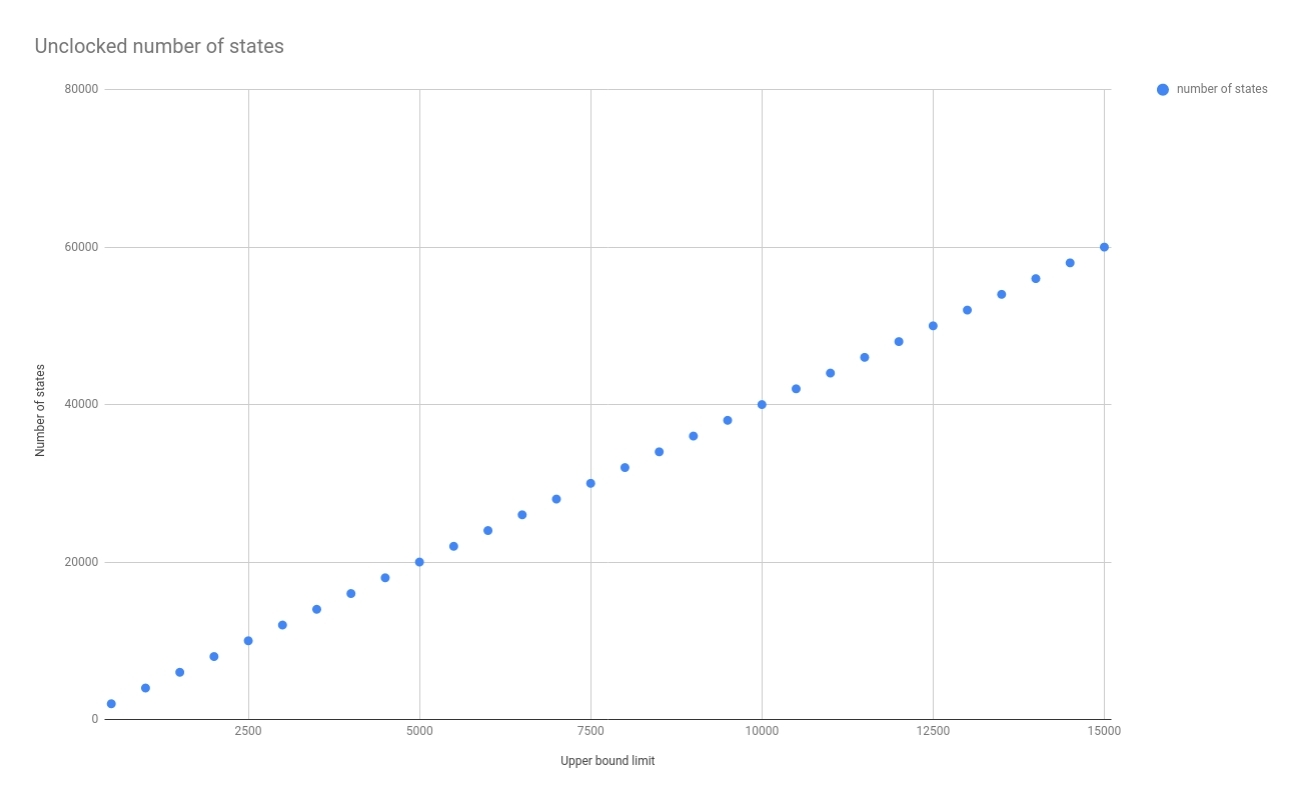
\includegraphics[width=0.98\textwidth]{./figures/15-11-2018/unclocked_number_of_states.jpg}
\caption{y}
\label{fig:unclocked_states}
\end{figure}
\paragraph{Verification time}
In Figure \ref{fig:unclocked_verification}the verification time results can be seen. The graph represents the verification time in seconds for each increase of the input range. As can be seen the verification time increase exponentially with the input values. Since the number of states are increasing linearly it can seem odd that the verification time does not follow that same pattern. However, besides the refinement checking of the GLTS which will increase with the number of states, FDR4 must compile the network and generate the GLTS. It is reasonable to expect that the larger the state space, the more effort for FDR4 to complete all the steps of the verification. Therefore these results are consistent with what could be expected.
\begin{figure}
    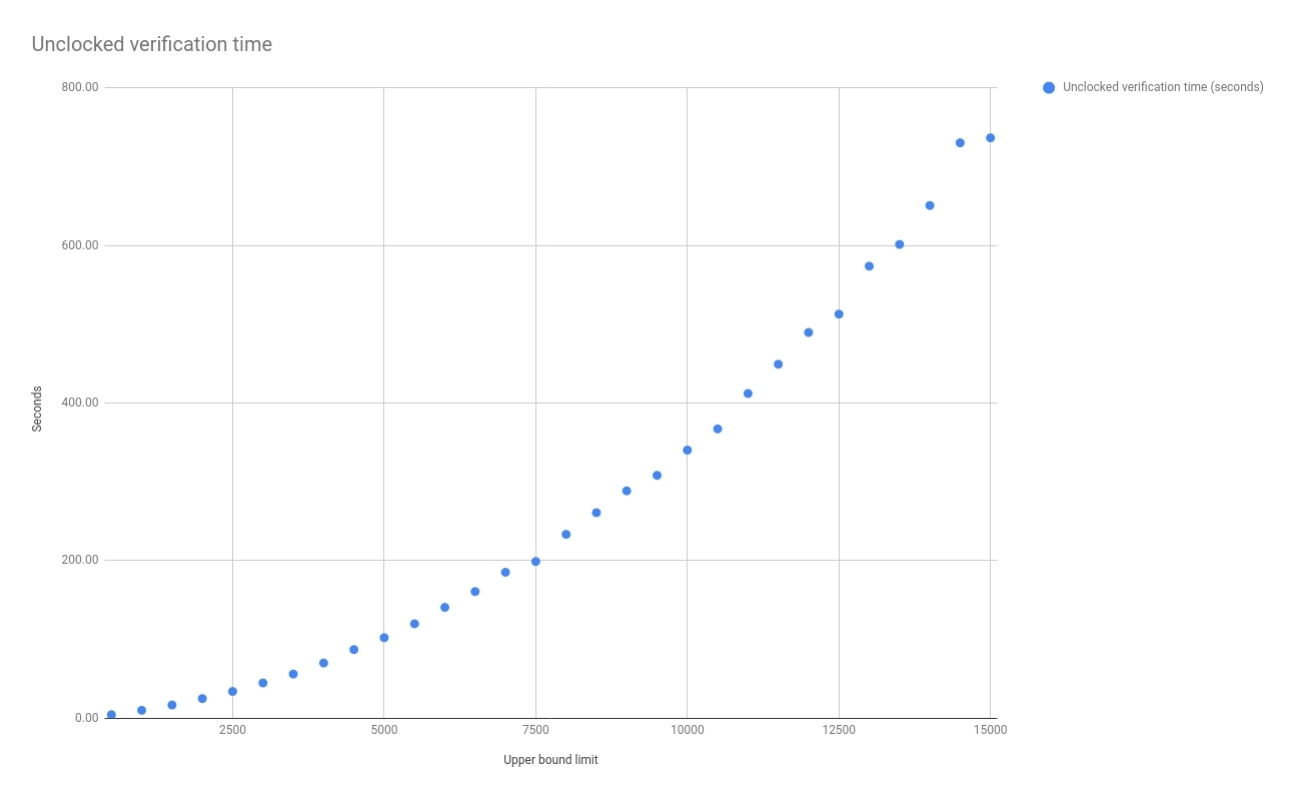
\includegraphics[width=0.98\textwidth]{./figures/15-11-2018/unclocked_verification_time.jpg}
\caption{x}
\label{fig:unclocked_verification}
\end{figure}
\paragraph{Maximum resident set size}
The result from this property can be seen in Figure \ref{fig:unclocked_resident_size}. These results are not fittet to a line as well as the other two experiment properties. It is clear that the amount of memory used for the verification grows with an increase in the input range. It is also somewhat consistent unil around 10000 in upper bound limit. This different could be caused by some internal structure in FDR4 or it could be a result of other requirements within the machine that is running the verification. Unfortunately FDR4 does not provide a lot of information about the internal workings and so it can be very difficult to examine these results further. However, these results are overall consistens with the results from both \texttt{number of states} and \texttt{verification time}.
\begin{figure}
    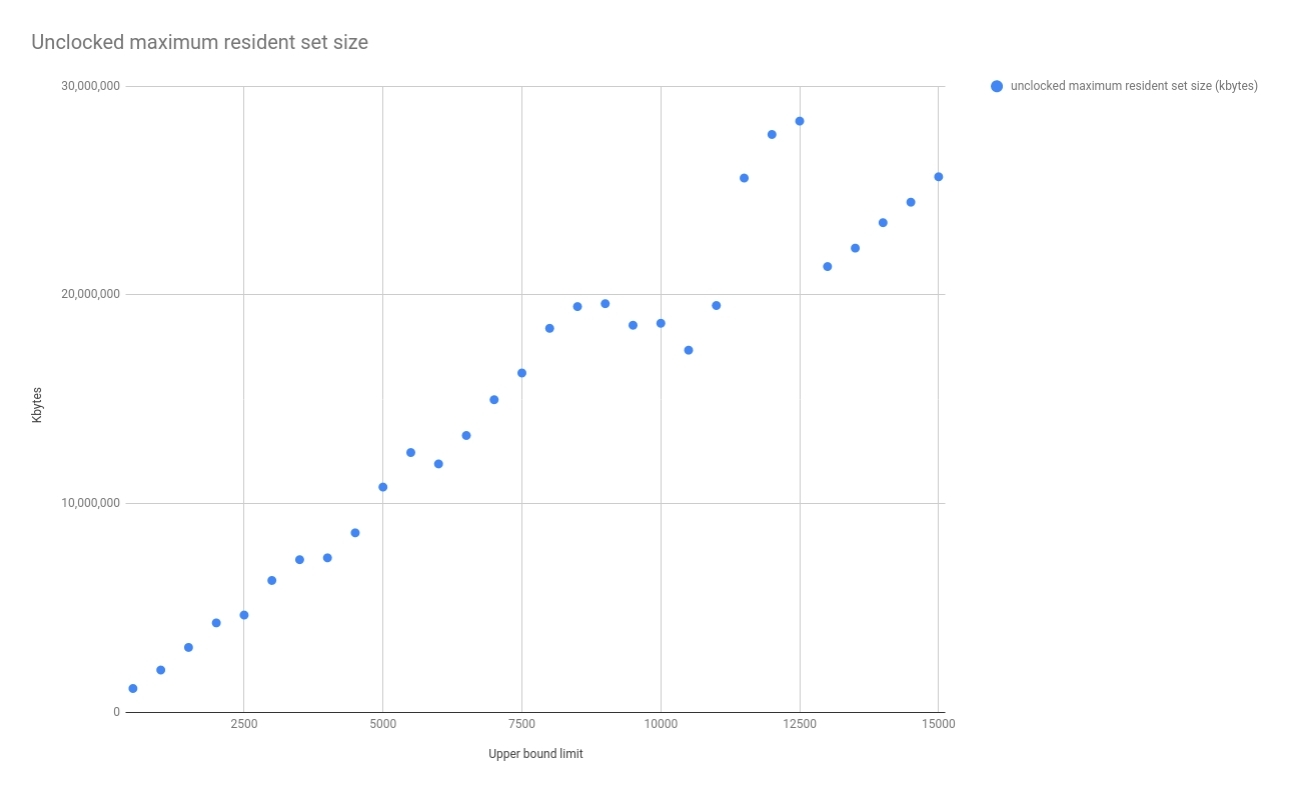
\includegraphics[width=0.98\textwidth]{./figures/15-11-2018/unclocked_maximum_resident_set_size.jpg}
\caption{y}
\label{fig:unclocked_resident_size}
\end{figure}


\subsection{Clocked Experiment}
% TODO when I know if I can use this example
\subsection{Results}
% TODO when I know I can use this example


\newpage
\section{How to use TAPS}
The required dependencies for generating the ANTLR4 parser, running TAPS and verifcation with FDR4 are listed below:
\begin{itemize}
    \item ANTLR4
    \item Python 2.7
    \item FDR4
\end{itemize}

ANTLR4 and FDR4 can both be downloaded from their websites where installation instructions are also provided.
ANTLR4 can be found at \url{https://www.antlr.org/} and FDR4 at \url{https://www.cs.ox.ac.uk/projects/fdr/}.\\
It is also necessary to download the Python runtime from \url{https://pypi.org/project/antlr4-python2-runtime/}.

Assuming that an ANTLR4 alias have been created as the ANTLR4 installation suggest, to generate the parser and lexer with ANTLR4 run {\ttfamily antlr4 -Dlanguage=Python2 - visitor -no-listener Smeil.g4.}
This will create all the required parser and lexer files as well as the visitor methods. This step is only necessary if the .g4 grammar file have been modified.\\

When the ANTLR4 files have been generated TAPS can be used directly with a well-formed SMEIL program with the command: {\ttfamily python taps.py input.sme output.csp}. The system requires both an input file as well as an output file. If the output file does not exists it will be created by TAPS. \\

The resulting \cspm{} file can be verified in FDR either by the command line tool or by the FDR4 tool which is a graphical tool. The command line tool can be used by the command \texttt{refines output.csp}. There are several options to adjust the output of the command. The FDR4 command line tool is mostly used to quickly check if a network pass the verification because it is difficult to navigate the counter examples. The FDR4 graphical tool provides a better visualisation of counter examples and the ProBE visualiser can be called directly from the FDR graphical tool.

